\section*{\Large{Введение}}
В современном мире каждая компания хочет минимизировать свои
затраты, как по времени, так и в финансовом плане.
Это не обошло и сферу строительства.
В данной области существует ряд открытых задач, требующих решения,
в том числе это касается сферы проектирования генеральных планов площадных объектов.


Любоe сооружение несет в себе определенную функцию. Склады служат для хранения вещей, факелы для сжигания
попутного газа, а нефтеперерабатывающий завод для преобразования сырой нефти в нефтепродукты.
Чем сложнее задача, которую решает промышленный объект,
тем сложнее он устроен, и из большего числа сооружений он состоит.
А чем больше сооружений находится рядом, тем больше появляется различных ограничений,
продиктованных вопросами безопасности строительства этих зданий рядом.

\begin{figure}[H]
	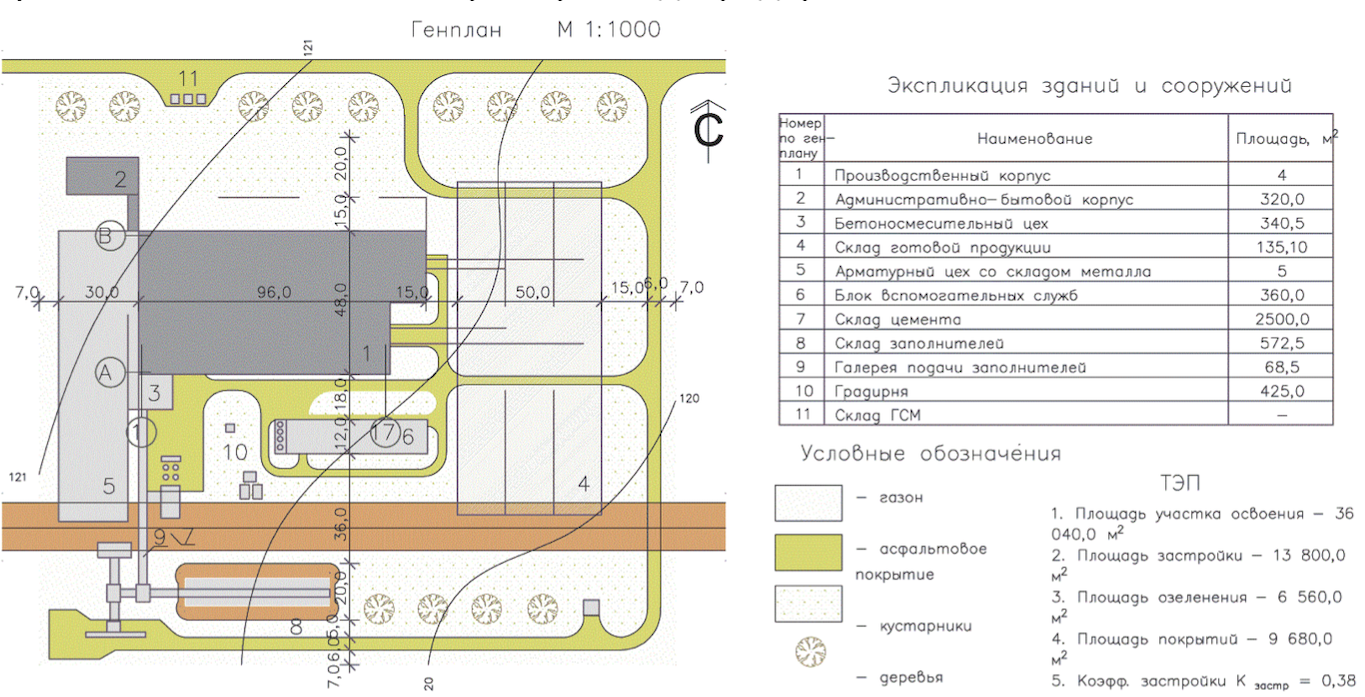
\includegraphics[width=0.9\textwidth]{images/introduction/1}
	\caption{Генеральный план завода}
	\label{pic:introduction__site_plan}
\end{figure}
\vskip 5 mm

Крайне опасно размещать факел для сжигания попутного рядом с хранилищем топлива из-за высокой пожароопасности хранилища.
В случае возгорания хранилища, топливо, которое находится в нём, может быть не только огнеоопасным, но также
и взрывоопасным. Соответственно, если в зоне поражения взрыва находятся сооружения, требующие постоянного присутствия людей,
то помимо повреждения материальных объектов, могут погибнуть или быть травмированы люди, чего допускать никак нельзя.


Проектирование генерального плана промышленного сооружения служит, как раз для того,
чтобы минимизировать риски возникновения нештатных ситуаций, повреждения материального имущества, а также, что
наиболее важно, риск возникновения несчастных случаев на предприятии.


Также очень важно учитывать не только взаимодействие зданий внутри промышленного объекта, но и учитывать
характеристики местности, где этот объект будет построен. Характеристики местности очень разнообразны и включают в себя
не только физические величины, такие как объем грунта при разравнивании площадки и общую длину ограждения вокруг объекта,
так и различные юридические аспекты, будь то уровень загрязнения окружающей среды или уровень производимого шума.
